
%<<setup-child, include = FALSE>>=

%library(knitr)
%options(digits = 16)

%library(RCurl)
%library(XML)
%library(tm)
%library(NMF)
%library(microbenchmark)
%library(ggplot2)
%library(wordcloud)
%set_parent("../style/preamble.Rnw")
%@


\newcommand{\xdownarrow}[1]{%
	{\left\downarrow\vbox to #1{}\right.\kern-\nulldelimiterspace}
}

\newcommand{\grey}[1]{\textcolor{grey}{#1}}
\newcommand{\red}[1]{\textcolor{red}{#1}}

\input{../../2021/style/preamble4tex}
% dependencies: amsmath, amssymb, dsfont
% math spaces
\ifdefined\N
\renewcommand{\N}{\mathds{N}} % N, naturals
\else \newcommand{\N}{\mathds{N}} \fi
\newcommand{\Z}{\mathds{Z}} % Z, integers
\newcommand{\Q}{\mathds{Q}} % Q, rationals
\newcommand{\R}{\mathds{R}} % R, reals
\ifdefined\C
\renewcommand{\C}{\mathds{C}} % C, complex
\else \newcommand{\C}{\mathds{C}} \fi
\newcommand{\continuous}{\mathcal{C}} % C, space of continuous functions
\newcommand{\M}{\mathcal{M}} % machine numbers
\newcommand{\epsm}{\epsilon_m} % maximum error

% counting / finite sets
\newcommand{\setzo}{\{0, 1\}} % set 0, 1
\newcommand{\setmp}{\{-1, +1\}} % set -1, 1
\newcommand{\unitint}{[0, 1]} % unit interval

% basic math stuff
\newcommand{\xt}{\tilde x} % x tilde
\newcommand{\argmin}{\mathop{\mathrm{arg\,min}}} % argmin
\newcommand{\argmax}{\mathop{\mathrm{arg\,max}}} % argmax
\newcommand{\argminlim}{\argmin\limits} % argmin with limits
\newcommand{\argmaxlim}{\argmax\limits} % argmax with limits
\newcommand{\sign}{\operatorname{sign}} % sign, signum
\newcommand{\I}{\mathbb{I}} % I, indicator
\newcommand{\order}{\mathcal{O}} % O, order
\newcommand{\bigO}{\mathcal{O}} % Big-O Landau
\newcommand{\littleo}{{o}} % Little-o Landau
\newcommand{\pd}[2]{\frac{\partial{#1}}{\partial #2}} % partial derivative
\newcommand{\floorlr}[1]{\left\lfloor #1 \right\rfloor} % floor
\newcommand{\ceillr}[1]{\left\lceil #1 \right\rceil} % ceiling
\newcommand{\indep}{\perp \!\!\! \perp} % independence symbol

% sums and products
\newcommand{\sumin}{\sum\limits_{i=1}^n} % summation from i=1 to n
\newcommand{\sumim}{\sum\limits_{i=1}^m} % summation from i=1 to m
\newcommand{\sumjn}{\sum\limits_{j=1}^n} % summation from j=1 to p
\newcommand{\sumjp}{\sum\limits_{j=1}^p} % summation from j=1 to p
\newcommand{\sumik}{\sum\limits_{i=1}^k} % summation from i=1 to k
\newcommand{\sumkg}{\sum\limits_{k=1}^g} % summation from k=1 to g
\newcommand{\sumjg}{\sum\limits_{j=1}^g} % summation from j=1 to g
\newcommand{\summM}{\sum\limits_{m=1}^M} % summation from m=1 to M
\newcommand{\meanin}{\frac{1}{n} \sum\limits_{i=1}^n} % mean from i=1 to n
\newcommand{\meanim}{\frac{1}{m} \sum\limits_{i=1}^m} % mean from i=1 to n
\newcommand{\meankg}{\frac{1}{g} \sum\limits_{k=1}^g} % mean from k=1 to g
\newcommand{\meanmM}{\frac{1}{M} \sum\limits_{m=1}^M} % mean from m=1 to M
\newcommand{\prodin}{\prod\limits_{i=1}^n} % product from i=1 to n
\newcommand{\prodkg}{\prod\limits_{k=1}^g} % product from k=1 to g
\newcommand{\prodjp}{\prod\limits_{j=1}^p} % product from j=1 to p

% linear algebra
\newcommand{\one}{\bm{1}} % 1, unitvector
\newcommand{\zero}{\mathbf{0}} % 0-vector
\newcommand{\id}{\bm{I}} % I, identity
\newcommand{\diag}{\operatorname{diag}} % diag, diagonal
\newcommand{\trace}{\operatorname{tr}} % tr, trace
\newcommand{\spn}{\operatorname{span}} % span
\newcommand{\scp}[2]{\left\langle #1, #2 \right\rangle} % <.,.>, scalarproduct
\newcommand{\mat}[1]{\begin{pmatrix} #1 \end{pmatrix}} % short pmatrix command
\newcommand{\Amat}{\mathbf{A}} % matrix A
\newcommand{\Deltab}{\mathbf{\Delta}} % error term for vectors

% basic probability + stats
\renewcommand{\P}{\mathds{P}} % P, probability
\newcommand{\E}{\mathds{E}} % E, expectation
\newcommand{\var}{\mathsf{Var}} % Var, variance
\newcommand{\cov}{\mathsf{Cov}} % Cov, covariance
\newcommand{\corr}{\mathsf{Corr}} % Corr, correlation
\newcommand{\normal}{\mathcal{N}} % N of the normal distribution
\newcommand{\iid}{\overset{i.i.d}{\sim}} % dist with i.i.d superscript
\newcommand{\distas}[1]{\overset{#1}{\sim}} % ... is distributed as ...


\begin{document}

\lecturechapter{7}{Non-Negative Matrix Factorization \& Recommender Systems Application}
\lecture{CIM1 Statistical Computation}



\begin{vbframe}{Non-negative matrix factorization}

This leads to a constrained optimization problem 

\begin{eqnarray*}
 \min_{\mathbf{W}\in \R^{m \times k}, \mathbf{H}\in \R^{k \times n}} & & \|\mathbf{X} - \mathbf{WH}\|^2, \\
\text{with } & & \mathbf{W} \ge 0, \mathbf{H} \ge 0
\end{eqnarray*}

The following problems must be addressed

\begin{enumerate}
\item NMF is NP-hard
\item NMF is ill-posed
\item Choice of rank $k$
\end{enumerate}

\framebreak

\begin{enumerate}
\item NMF is NP-hard \\

The problem is only convex in either $\mathbf{W}$ or $\mathbf{H}$, but not in both simultaneously. Probably there is no efficient, exact solution for NMF. There are efficient heuristics such as \textbf{multiplicative update rules}, but convergence to a global optimum cannot be guaranteed.

\begin{algorithm}[H]
  \caption{Multiplicative Update Rules}
  \begin{algorithmic}[1]
  \State Initialize $\mathbf{W}, \mathbf{H} \ge \mathbf{0}$
  \Repeat
    \State $h_{ij} \leftarrow h_{ij} \frac{(\mathbf{W^TX})_{ij}}{(\mathbf{W^TWH})_{ij}}$
    \State $w_{ij} \leftarrow w_{ij} \frac{(\mathbf{XH^T})_{ij}}{(\mathbf{WHH^T})_{ij}}$
  \Until Stop criterion fulfilled
  \end{algorithmic}
\end{algorithm}

\framebreak

\item NMF is ill-posed \\

\lz

The problem can usually not be solved uniquely.

\begin{eqnarray*}
\begin{pmatrix} 0 & 1 & 1 & 1 \\
1 & 0 & 1 & 1 \\
1 & 1 & 0 & 1 \end{pmatrix} &=& \begin{pmatrix} 0 & 1 & 1  \\
1 & 0 & 1 \\
1 & 1 & 0 \end{pmatrix} \begin{pmatrix} 1 & 0 & 0 & 0.5 \\
0 & 1 & 0 & 0.5 \\
0 & 0 & 1 & 0.5 \end{pmatrix} \\ &=&
\begin{pmatrix} 1 & 0 & 0  \\
0 & 1 & 0 \\
0 & 0 & 1 \end{pmatrix} \begin{pmatrix} 0 & 1 & 1 & 1 \\
1 & 0 & 1 & 1 \\
1 & 1 & 0 & 1 \end{pmatrix}
\end{eqnarray*}

Different factorizations mean different interpretations. Therefore in practice a regularization term is often added to the target function.

\framebreak

\item Choice of rank $k$

\lz

In contrast to singular value decomposition, it is much more difficult to determine the rank $k$ in advance.

\lz

Possibilities:

\begin{itemize}
\item $k$ is fixed in advance (based on prior knowledge / intuition) or results for different $k$ are compared
\item $k$ is automatically estimated during NMF (not discussed here)
\end{itemize}

\end{enumerate}

\end{vbframe}

\begin{vbframe}{Application: Recommender Systems (2)}

Back to our previous \textbf{example}:

\begin{footnotesize}
\begin{center}
\[
\begin{blockarray}{ccccc}
& \text{Die Hard} & \text{Top Gun} & \text{Titanic} &  \text{Notting Hill} \\
\begin{block}{r(cccc)}
\text{User 1} &  5  &  \textcolor{red}{\text{NA}}  & 3 &  \textcolor{red}{\text{NA}}  \\
\text{User 2}  & 5 & 4 & 3 &  3  \\
\text{User 3}  &  2  &  \textcolor{red}{\text{NA}}  & 5 &  \textcolor{red}{\text{NA}}  \\
\text{User 4}  & 5  &  5  &  3  &  1 \\
\text{User 5}  & 1  &  2  &  5  &  5  \\
\text{User 6}  & 1  &  2  &  4  &  5  \\
\end{block}
\end{blockarray}
 \]
\end{center}
\end{footnotesize}

Non-negative matrix factorization offers an alternative to singular value decomposition. The advantage of a NMF solution is the increased interpretability of the matrices $\mathbf{W}$ and $\mathbf{H}$.

\framebreak

\begin{enumerate}
\item We replace missing values with the row mean value:
%<<echo = F>>=
%options(digits = 2)
%@


%<<echo = F>>=
%X = t(matrix(c(5, NA, 3, NA,
%              5, 4, 3, 3,
%              2, NA, 5, NA,
%              5, 5, 3, 1,
%              1, 2, 5, 5,
%              1, 2, 4, 5), ncol = 6))

%movies = c("Die Hard", "Top Gun", "Titanic", "Notting Hill")
%colnames(X) = movies

%users = c("User 1", "User 2", "User 3", "User 4", "User 5", "User 6")
%rownames(X) = users
%@

%<<echo = F>>=
%X = ifelse(is.na(X), rowMeans(X, na.rm = TRUE), unlist(X))
%@

\item Choice of $k$:

\lz

We suspect that our movie database contains movies from two different categories and set $k=2$.

\lz

\item Non-negative matrix factorization:
\vspace{0.3cm}
\footnotesize

\begin{verbbox}
set.seed(1)
res = nmf(X, rank = 2)
W = res@fit@W
H = res@fit@H
\end{verbbox}
\col

\framebreak

%<<>>=
%set.seed(1)
%res = nmf(X, rank = 2)

%W = res@fit@W
%H = res@fit@H
%@

%<<echo = F>>=
%colnames(W) = c("Action", "Romance")

%rownames(H) = c("Action", "Romance")
%@

%<<>>=
%W
%@

%<<>>=
%H
%@

\begin{verbatim}
W
##           Action   Romance
## User 1     3.86     1.861
## User 2     4.06     1.360
## User 3     1.83     2.978
## User 4     5.14     0.098
## User 5     0.38     3.918
## User 6     0.44     3.540
\end{verbatim}

\lz 

\begin{verbatim}
H
##          Die Hard   Top Gun   Titanic   Notting Hill
## Action     1.08      0.91      0.46        0.22
## Romance    0.14      0.46      1.15        1.32
\end{verbatim}

\framebreak

\normalsize
The columns of the $6 \times 2$ matrix $\mathbf{W}$ could be interpreted as movie categories (here: \enquote{Action} and \enquote{Romance}). The figure shows which users prefer which categories.

\lz

\begin{center}
	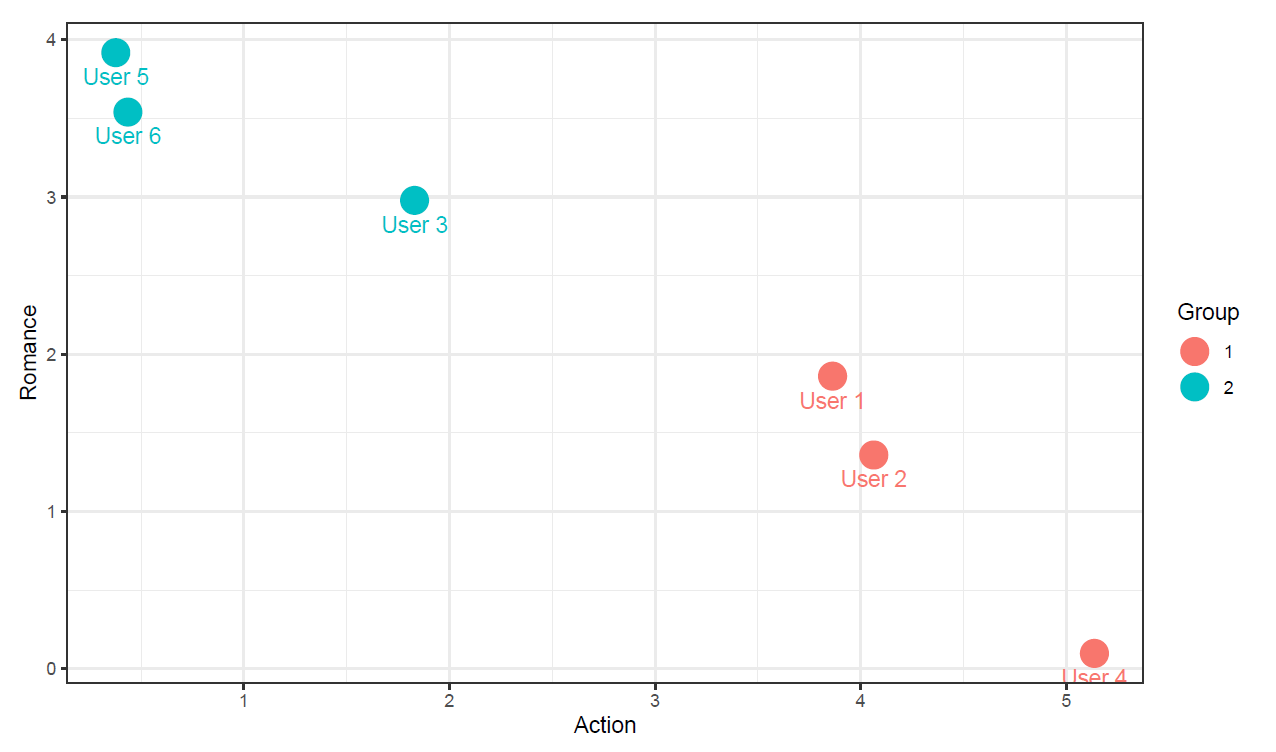
\includegraphics[width = 0.7\textwidth]{figure_man/recom-system-1.png}
\end{center}

%<<echo = F, out.width='80%', fig.align='center'>>=
%W.df = as.data.frame(W)
%W.df$Group = as.factor(c(1, 1, 2, 1, 2, 2))

%ggplot(data = W.df, aes(x = Action, y = Romance, col = Group, label = rownames(W.df))) + geom_point(size = 6) + geom_text(vjust = 2) + theme_bw()
%@

\framebreak

The entries of the $2 \times 4$ matrix $\mathbf{H}$ describe which movies are to be assigned to which category.

\lz

\begin{center}
	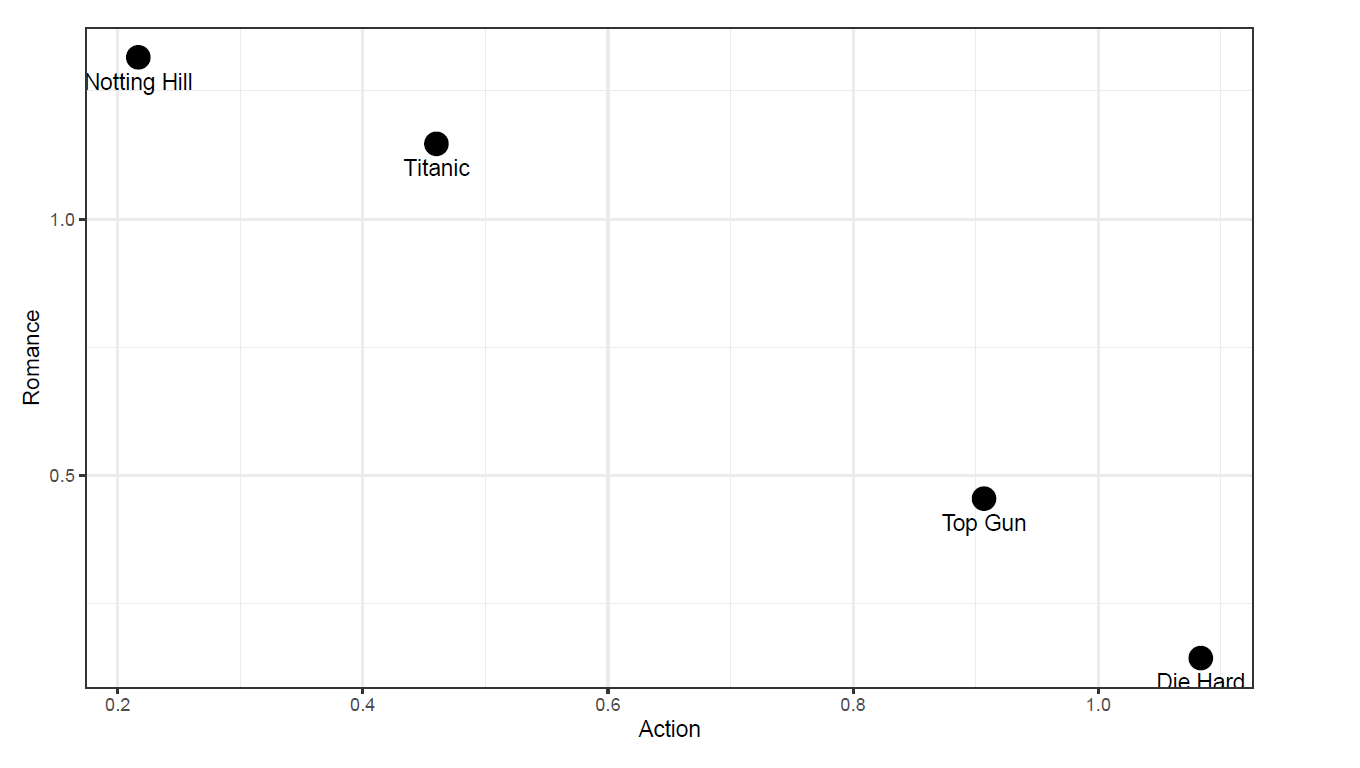
\includegraphics[width = 0.7\textwidth]{figure_man/recom-system-2.png}
\end{center}


%<<echo = F, fig.align='center', out.width='80%'>>=
%H.df = as.data.frame(t(H))

%ggplot(data = H.df, aes(x = Action, y = Romance, p, label = rownames(H.df))) + geom_point(size = 5) + geom_text(vjust = 2) + theme_bw()
%@
\framebreak

\item Calculate $\boldsymbol{\hat\mathbf{X}} = \mathbf{WH}$:

\footnotesize
\begin{verbatim}
W %*% H

##           Die Hard   Top Gun   Titanic   Notting Hill
## User 1      4.45      4.3        3.9        3.3
## User 2      4.60      4.3        3.4        2.7
## User 3      2.41      3.0        4.3        4.3
## User 4      5.58      4.7        2.5        1.2
## User 5      0.97      2.1        4.7        5.2
## User 6      0.98      2.0        4.3        4.8
\end{verbatim}

%<<>>=
%W %*% H
%@

\normalsize
Here we would also recommend \enquote{Top Gun} to user 1, an action movie. For user 3 we recommend \enquote{Notting Hill}, because he tends to prefer romantic movies.


\end{enumerate}


\end{vbframe}

\begin{vbframe}{More material on Recommender Systems}

More on Recommender Systems:
\begin{itemize}
\item \href{https://endymecy.gitbooks.io/spark-ml-source-analysis/content/\%E6\%8E\%A8\%E8\%8D\%90/papers/Matrix\%20Factorization\%20Techniques\%20for\%20Recommender\%20Systems.pdf}{Matrix Factorization Techniques for Recommender Systems}
\item \href{https://rpubs.com/tarashnot/recommender_comparison}{Recommender Systems Comparison (including implementation in R)}
\item \href{https://grouplens.org/datasets/movielens/100k/}{Movielens Dataset}
\end{itemize}

\end{vbframe}



\endlecture
\end{document}







